% LaTeX resume using res.cls
\documentclass{res}
%\usepackage{helvetica} % uses helvetica postscript font (download helvetica.sty)
%\usepackage{newcent}   % uses new century schoolbook postscript font  
\usepackage{graphicx}
\usepackage[hidelinks]{hyperref}
\graphicspath{ {images/} }
\setlength{\topmargin}{-0.6in}  % Start text higher on the page 
\setlength{\textheight}{9.8in}  % increase textheight to fit more on a page
\setlength{\headsep}{0.2in}     % space between header and text
\setlength{\headheight}{12pt}   % make room for header
\usepackage{fancyhdr}  % use fancyhdr package to get 2-line header
\renewcommand{\headrulewidth}{0pt} % suppress line drawn by default by fancyhdr
\lhead{\hspace*{-\sectionwidth}Teleport Security Model} % force lhead all the way left
\rhead{Page \thepage}  % put page number at right
\cfoot{}  % the footer is empty
\pagestyle{fancy} % set pagestyle for the document

\begin{document} 
\thispagestyle{empty} % this page does not have a header
\name{Teleport Security Model}


\begin{resume}
\vspace{0.1in}

\section{Intro}
\vspace{0.1in} 
 
   Teleport is an SSH server that supports only short lived certificates as authentication method.
   It provides two ways to access the cluster - via SSH or web-based access.

\section{Components}
\vspace{0.1in}

    Teleport system consists of two independent parts:

    \begin{itemize} %
      \item Teleport Cluster is a set of remote SSH servers using one host certificate authority to identify the cluster.
      \item Teleport Proxy is a remote SSH proxy that uses user certificate authority to identify the organization and is set up remotely and indepenedently from the Teleport Cluster.
    \end{itemize}

 
    Teleport proxy and teleport cluster identify each other by trusting each other keys used as a certificate authorities:

    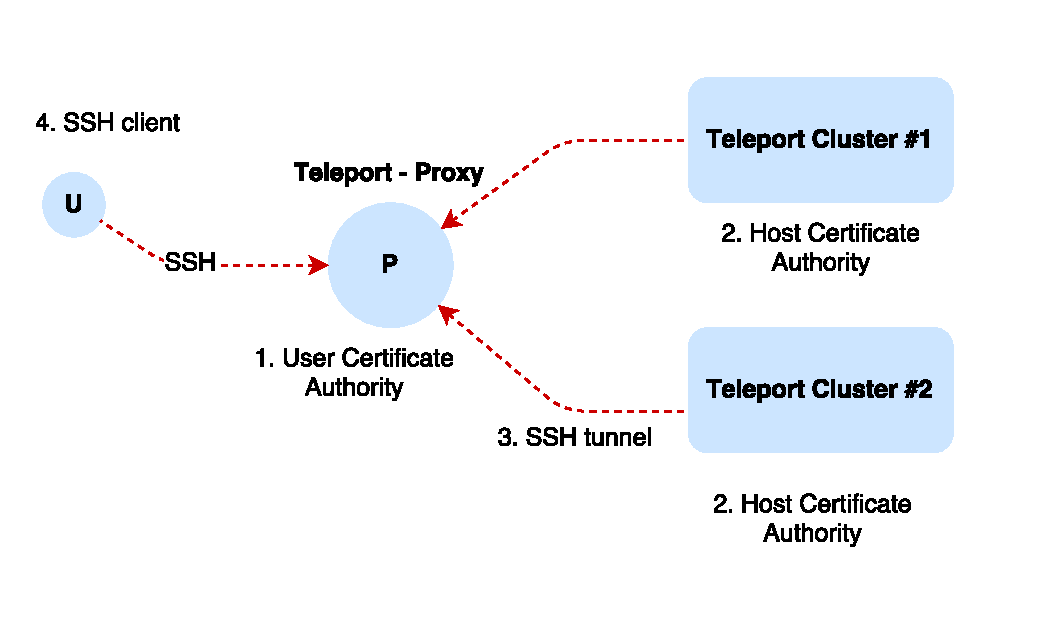
\includegraphics[scale=0.8]{./images/teleport-proxy-cluster.pdf}

    \begin{enumerate} %
      \item Teleport-proxy uses certs signed by it's user certificate authority to identify it's users. Teleport-proxy has a list of trusted remote host certificate authorities, keys signed by these authorities ar the only keys that are allowed to connect to it.
      \item Teleport-cluster uses host certs signed by it's host certificate authority to identify SSH tunnel connections mantained by some of it's tunnel servers.
      \item Teleport-cluster initiates and mantains the SSH tunnel to the teleport-proxy that is used for all SSH communications between users and the remote cluster.
      \item Individual SSH clients connect to Teleport-Proxy to connect to remote teleport clusters.    
    \end{enumerate}

    It's worth to mention that as long as teleport-cluster initiates the connection to the proxy, it does not have the listening socket, and the possible attack vector is shifted from the remote infrastructure to the teleport-proxy.

    This model allows teleport-cluster not to care about the users of every organization and sub organization that has access to it's servers. Teleport-proxy can implement it's own LDAP or any other ACL rules to give/revoke access to every cluster.

    Not every server has to connect to the teleport-proxy. Teleport cluster is capable of proxying the connection to any server in the cluster using agent-forwarding if it's allowed by the SSH client.

\section{Web access}
\vspace{0.1in}

    Teleport-proxy users can use Web access that uses 2-Factor auth to grant access to the remote clusters:
 
    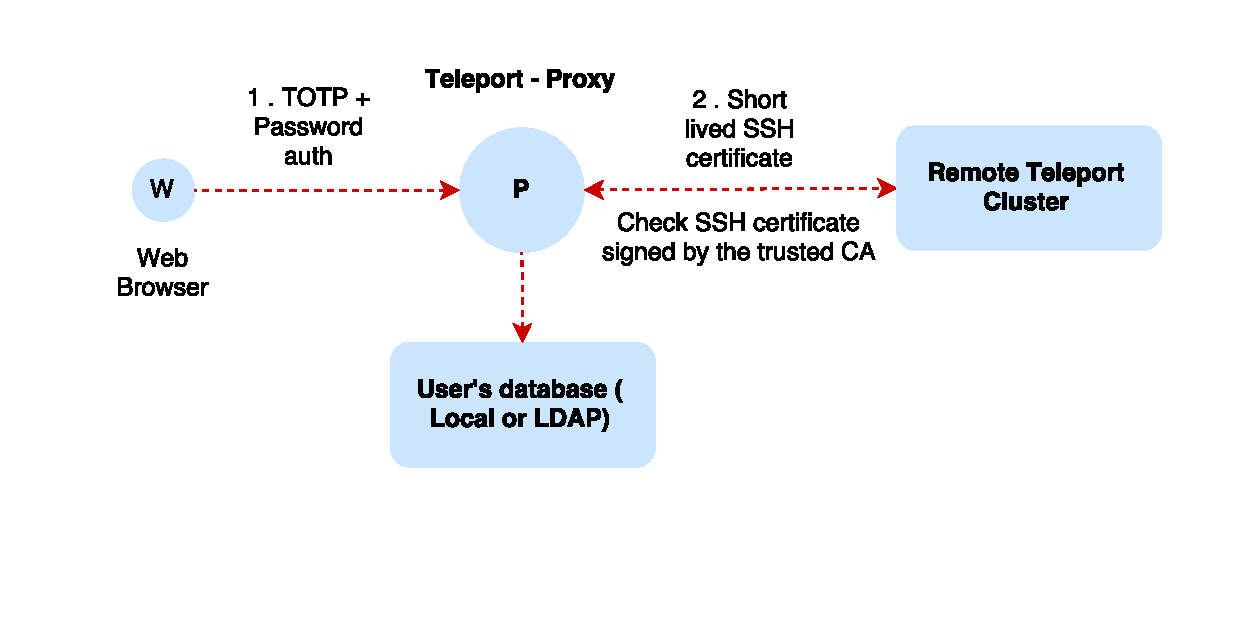
\includegraphics[scale=0.8]{./images/teleport-web.pdf}


    \begin{enumerate} %
      \item Teleport-proxy uses 2-Factor auth (password and TOTP keys as a second factor) to authenticate user.
      \item Teleport-proxy generates a short-lived key-pair signed by it's certificate authority and associates this key pair with user's web session. Later on it acts as SSH agent on behalf of user session to authenticate within the remote cluster. It uses web sockets to proxy terminal interaction with the remote cluster and initiates the connecton to the remote teleport cluster.
      \item Teleport-cluster checks the certificate just as any other SSH connection.
    \end{enumerate}

    As long as web session expires in about an hour, the key-pair get's deleted.

\section{SSH access}
\vspace{0.1in}

    Teleport-proxy users can use standard SSH client access that uses teleport-proxy as a proxying SSH server to connect to the remote clusters:
 
    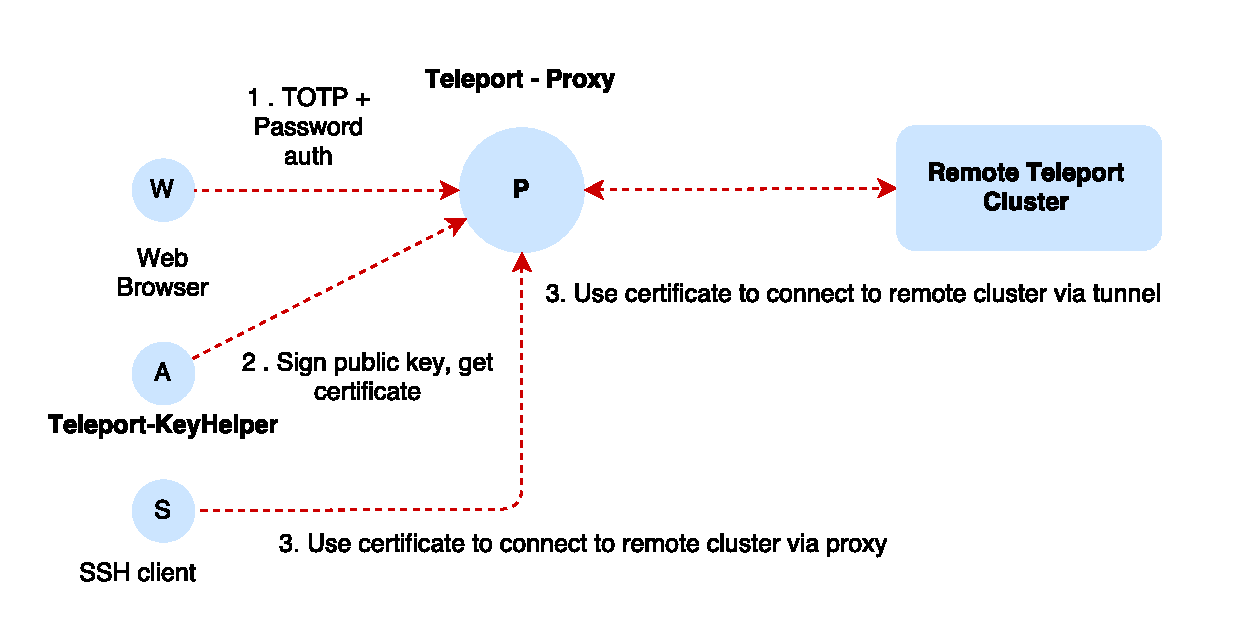
\includegraphics[scale=0.8]{./images/teleport-ssh.pdf}

    \begin{enumerate} %
      \item Users use the same 2-factor auth to gain access to the cluster. 
      \item Teleport-Keyhelper is a small utility program that mantains a persistent TLS connection to the teleport-proxy. It uses private key over TLS to identify itself. Once it detects that the user has signed in, it sends a user's public key for teleport-proxy to sign. Once the key is signed it writes the certificate to the desired destination.
      \item SSH client uses the new key to connect to the teleport-proxy.
    \end{enumerate}

    A bit more on the teleport-keyhelper. This is a small utility program that helps to get a signed certificate fromt he teleport-proxy and update
    it on the host, to reduce friction for the end user, user does not have to copy-paste the new certificate each time after sign-on was successful:
    \begin{verbatim}
      teleport-key-helper\
          --server=https://example.com/teleport-proxy
          --auth=username --token=token\    # token is used to grant access to this key-helper
          --key-path=/path-to-pubkey.pub\   # path to a public key to sign
          --cert-path=/path-to-cert.cert    # path to a key to overwrite
    \end{verbatim}

    This model will allow to use short-lived keys that are valid for a working day, so user will need to authorize only once a day
    and use both web and ssh access to the cluster.

    As long as certs are no longer valid after a short period of time, no revocation is necessary.

    If it's needed to terminate user access to the cluster, it's ACL entry in teleport can be deleted and regardless of the certificate
    user won't be able to access any teleport cluster.

\end{resume}
\end{document}































